%%%%%%%%%%%%%%%%%%%%%%%%%%%%%%%%%%%%%%%%%
% Beamer Presentation
% LaTeX Template
% Version 1.0 (10/11/12)
%
% This template has been downloaded from:
% http://www.LaTeXTemplates.com
%
% License:
% CC BY-NC-SA 3.0 (http://creativecommons.org/licenses/by-nc-sa/3.0/)
%
%%%%%%%%%%%%%%%%%%%%%%%%%%%%%%%%%%%%%%%%%

%----------------------------------------------------------------------------------------
%	PACKAGES AND THEMES
%----------------------------------------------------------------------------------------

\documentclass{beamer}

\mode<presentation> {

% The Beamer class comes with a number of default slide themes
% which change the colors and layouts of slides. Below this is a list
% of all the themes, uncomment each in turn to see what they look like.

%\usetheme{default}
%\usetheme{AnnArbor}
%\usetheme{Antibes}
%\usetheme{Bergen}
%\usetheme{Berkeley}
%\usetheme{Berlin}
%\usetheme{Boadilla}
%\usetheme{CambridgeUS}
%\usetheme{Copenhagen}
%\usetheme{Darmstadt}
%\usetheme{Dresden}
%\usetheme{Frankfurt}
%\usetheme{Goettingen}
%\usetheme{Hannover}
%\usetheme{Ilmenau}
%\usetheme{JuanLesPins}
%\usetheme{Luebeck}
\usetheme{Madrid}
%\usetheme{Malmoe}
%\usetheme{Marburg}
%\usetheme{Montpellier}
%\usetheme{PaloAlto}
%\usetheme{Pittsburgh}
%\usetheme{Rochester}
%\usetheme{Singapore}
%\usetheme{Szeged}
%\usetheme{Warsaw}

% As well as themes, the Beamer class has a number of color themes
% for any slide theme. Uncomment each of these in turn to see how it
% changes the colors of your current slide theme.

%\usecolortheme{albatross}
%\usecolortheme{beaver}
%\usecolortheme{beetle}
%\usecolortheme{crane}
%\usecolortheme{dolphin}
%\usecolortheme{dove}
%\usecolortheme{fly}
%\usecolortheme{lily}
%\usecolortheme{orchid}
%\usecolortheme{rose}
%\usecolortheme{seagull}
%\usecolortheme{seahorse}
%\usecolortheme{whale}
%\usecolortheme{wolverine}

%\setbeamertemplate{footline} % To remove the footer line in all slides uncomment this line
%\setbeamertemplate{footline}[page number] % To replace the footer line in all slides with a simple slide count uncomment this line

%\setbeamertemplate{navigation symbols}{} % To remove the navigation symbols from the bottom of all slides uncomment this line
}

\usepackage{graphicx} % Allows including images
\usepackage{booktabs} % Allows the use of \toprule, \midrule and \bottomrule in tables
\usepackage{amsmath}
\newcommand{\norm}[1]{\left\lVert#1\right\rVert}

%----------------------------------------------------------------------------------------
%	TITLE PAGE
%----------------------------------------------------------------------------------------

\title[Detecting Structure in Graphs]{Detecting Structure in Graphs } % The short title appears at the bottom of every slide, the full title is only on the title page

\author{Gautam Rayaprolu} % Your name
\institute[McGill University] % Your institution as it will appear on the bottom of every slide, may be shorthand to save space
{
McGill University \\ % Your institution for the title page
\medskip
\textit{gautam.rayaprolu@mail.mcgill.ca} % Your email address
}
\date{\today} % Date, can be changed to a custom date

\begin{document}

\begin{frame}
\titlepage % Print the title page as the first slide
\end{frame}

%\begin{frame}
%\frametitle{Overview} % Table of contents slide, comment this block out to remove it
%\tableofcontents % Throughout your presentation, if you choose to use \section{} and \subsection{} commands, these will automatically be printed on this slide as an overview of your presentation
%\end{frame}

%----------------------------------------------------------------------------------------
%	PRESENTATION SLIDES
%----------------------------------------------------------------------------------------

%------------------------------------------------
%\section{First Section} % Sections can be created in order to organize your presentation into discrete blocks, all sections and subsections are automatically printed in the table of contents as an overview of the talk
%------------------------------------------------

%\subsection{Subsection Example} % A subsection can be created just before a set of slides with a common theme to further break down your presentation into chunks

%------------------------------------------------

\begin{frame}
\frametitle{Introduction}
\begin{itemize}
\item An Erdos Renyi Random Graph $G(n,p)$ is a graph on $n$ vertices where each of the $n \choose 2$ edges exists independently with probability p
\item The largest clique on this graph is $O(log(n))$ with high probability
\item As part of this project I showed that the largest hypercube on this graph is $O(log(log(n)))$
\item You can use spectral methods to detect a planted clique of size atleast $O(\sqrt{n})$ on this graph
\end{itemize}
\end{frame}


\begin{frame}
\frametitle{Random Graphs as a model of networks}
\begin{itemize}
\item ER graphs have a low clustering coefficient and their degrees are distributed as a Poisson Distribution.
\item Many real world graphs have been shown to a power law degree distribution. i.e. $P(k) \approx k^{-\gamma}$
\item The clustering coefficient shows how close neighbours are to being a clique
\item Many models have been suggested, most notably the watts-strogatz small world graph
\end{itemize}
\end{frame}


%------------------------------------------------

\begin{frame}
\frametitle{Erdos Renyi Graph}
\begin{figure}
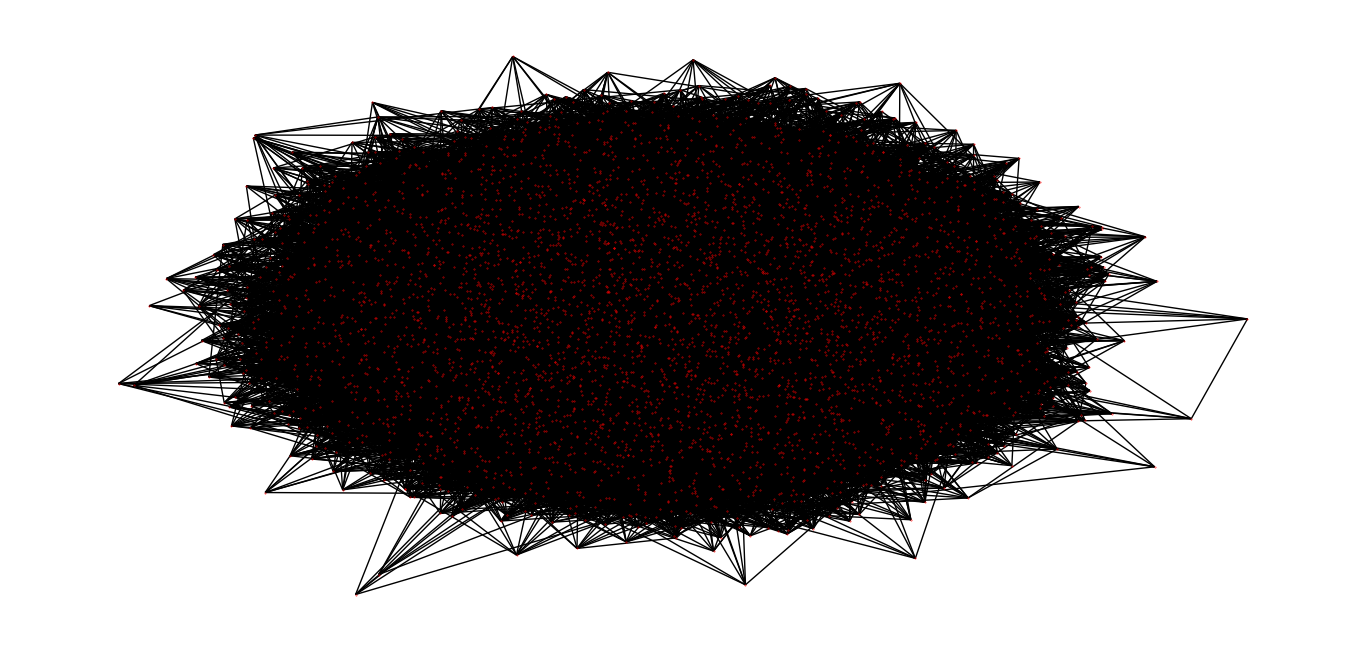
\includegraphics[width=\textwidth,height=\textheight,keepaspectratio]{Gnp_connectivity_graph}
\end{figure}
\end{frame}


\begin{frame}
\frametitle{Watts Strogatz Small World Graph}
\begin{figure}
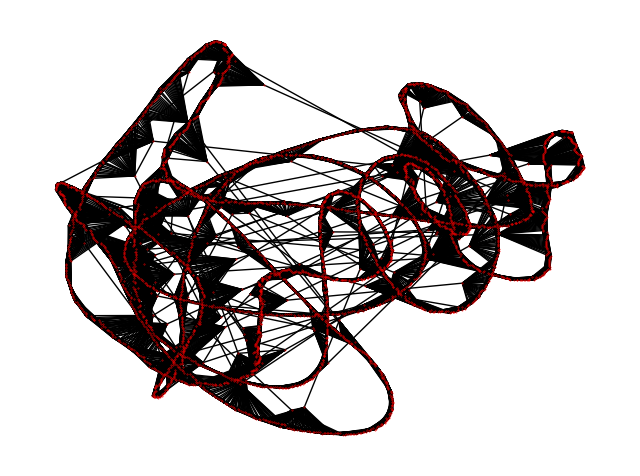
\includegraphics[width=\textwidth,height=\textheight,keepaspectratio]{watts_strogatz_connectivity_graph}
\end{figure}
\end{frame}


\begin{frame}
\frametitle{Facebook Network Graph}
\begin{figure}
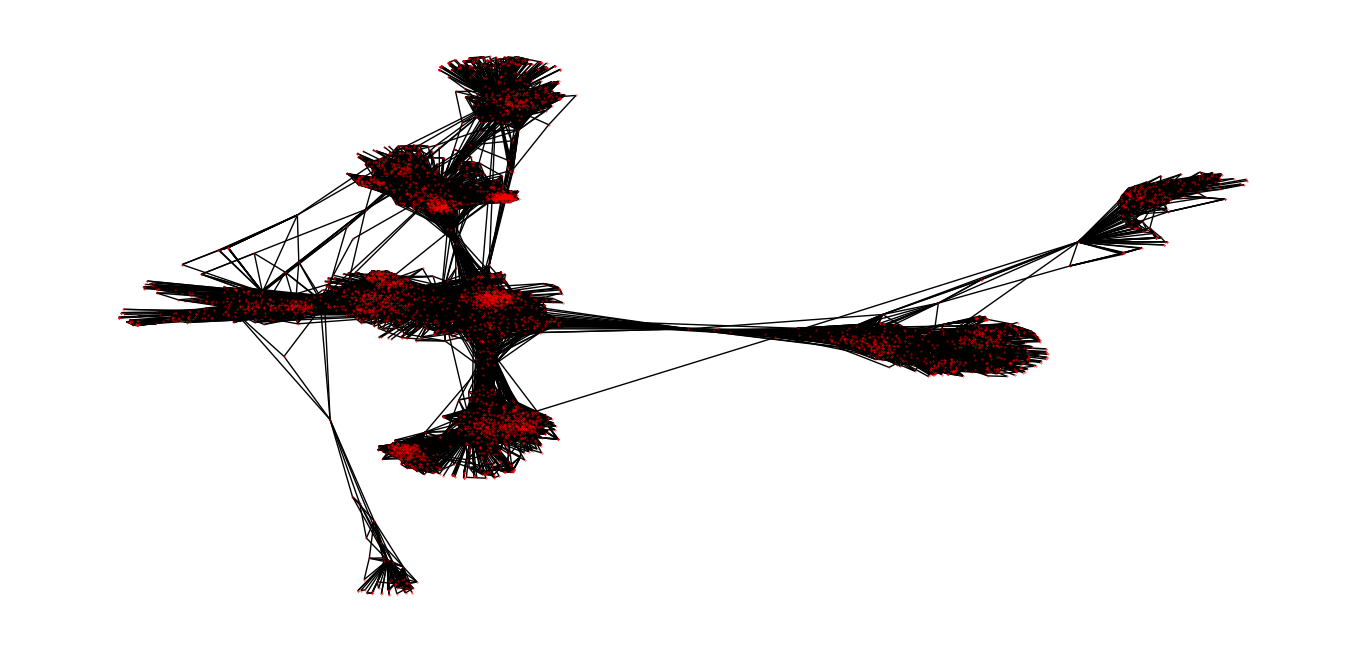
\includegraphics[width=\textwidth,height=\textheight,keepaspectratio]{facebook_connectivity_graph}
\end{figure}
\end{frame}

%------------------------------------------------

\begin{frame}
\frametitle{Kronecker Graphs}
\begin{itemize}
\item The Kronecker product of 2 matrices $A \otimes B$ is the process where each element $a_{ij}$ of $A$ is replaced by the matrix $a_{ij}B$
\item The adjacency matrix of a Kronecker graph is constructed by taking an 'initiator' adjacency matrix $P$ and repeatedly applying the Kronecker Product with itself
\item We could alternative take values between $0$ and $1$ and interpret them as probabilities of the edge occurring
\end{itemize}
\end{frame}

%potentially have a slide for showing how the kronecker product works

\begin{frame}
\frametitle{The KronFit Algorithm}
\begin{itemize}
\item This algorithm was described by \cite{ghahramani2010} in 2010
\item Given a graph $G$ with $N = N_1^k$ nodes we wish the compute a MLE estimator for the stochastic initiator matrix $P$ of size $N_1$
\item $log(l(\Theta)) = log(P(G|\Theta) = log \sum_{\sigma} P(G|\Theta, \sigma)P(\sigma)$ where sigma represents a permutation of labellings
\item Use Metropolis sampling to get an estimate of the sum , which has $N!$ terms.
\item Note that there are several global maxima corresponding to different permutations of the Initiator Matrix

\end{itemize}
\end{frame}

%------------------------------------------------

\begin{frame}
\frametitle{Optimizations}
\begin{itemize}
\item Naively Calculating the likelihood takes $O(N^2)$ time
\item For the metropolis sampling algorithm we uniformly pick 2 indices and swap the nodes at those indices with probability $\frac{P(\sigma^i|G,\Theta)}{P(\sigma^{i-1}|G,\Theta)}$
\item This difference only takes $O(N)$ to calculate
\item The adjacency matrix of the training graph is sparse, so we can also estimate the full likelihood in $O(|E|)$ time which is roughly linear for real world graphs
\end{itemize}
\end{frame}

\begin{frame}
\frametitle{Experimental Results}
\begin{itemize}
\item I implemented the Kronfit algorithm using scipy's TNC minimizer and used it to fit 1024 nodes on the facebook graph.
\item Due to performance constraints I had to restrict the number of permutation samples to 100
\item The average clustering coeffecient of the facebook graph was around $0.7$ but that of the kronecker graph was around $0.03$ which is very similar to a $G(n,p)$
\item The log likehood's on the training data were of the order of $10^{-4}$ and did not vary much with different training sets
\end{itemize}
\end{frame}


\begin{frame}
\frametitle{Learned Kronecker Graph}
\begin{figure}
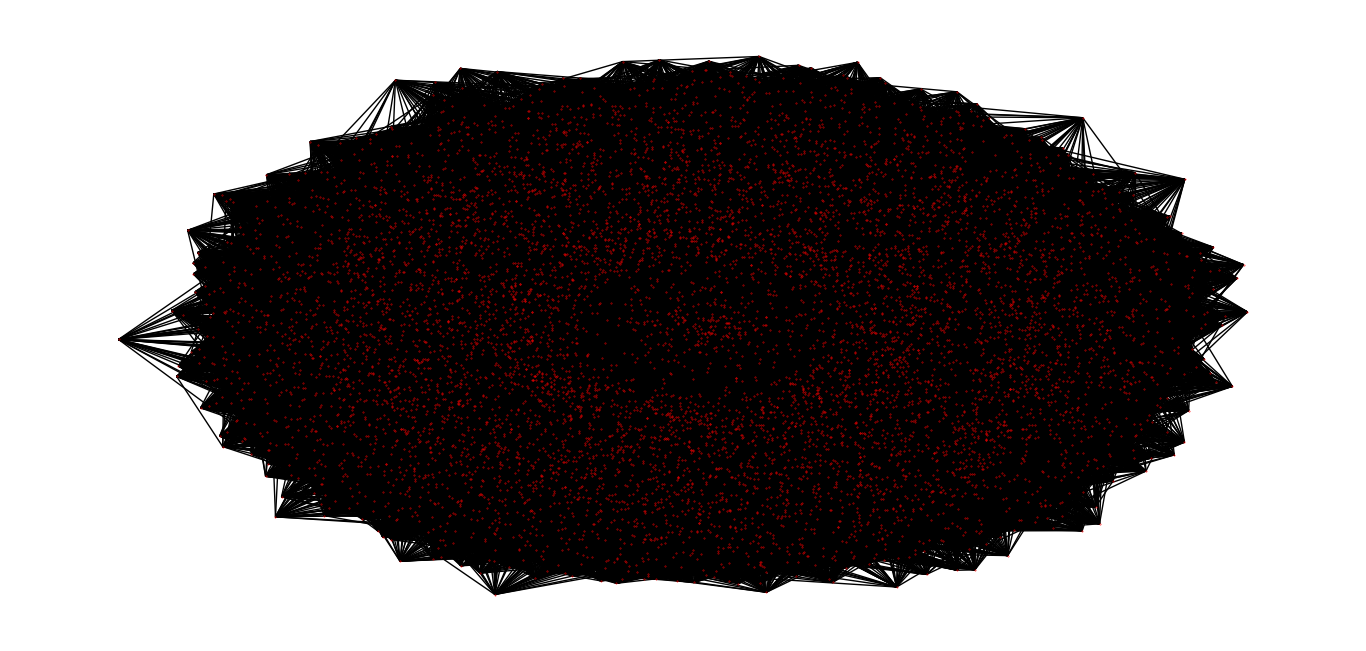
\includegraphics[width=\textwidth,height=\textheight,keepaspectratio]{kronecker_graph_P2}
\end{figure}
\end{frame}



\begin{frame}
\frametitle{Learned Kronecker Graph}
\begin{columns}[onlytextwidth]
\begin{column}{.45\textwidth}
\begin{figure}
  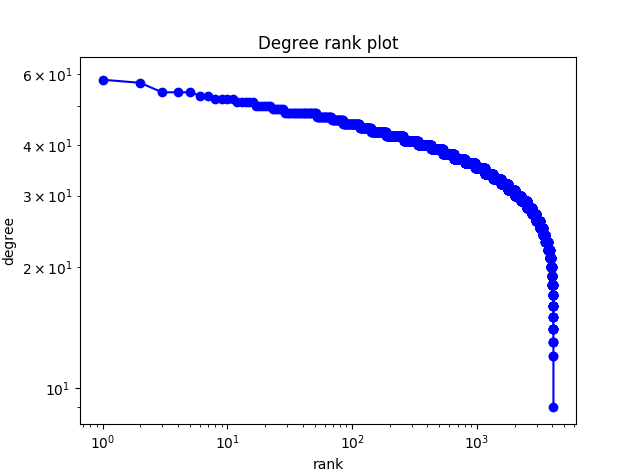
\includegraphics[width=\textwidth,height=\textheight,keepaspectratio]{kronecker_degree_distribution}\\
  \caption{Kronecker Degree Distribution}
\end{figure}
\end{column}
\hfill
\begin{column}{.45\textwidth}
\begin{figure}
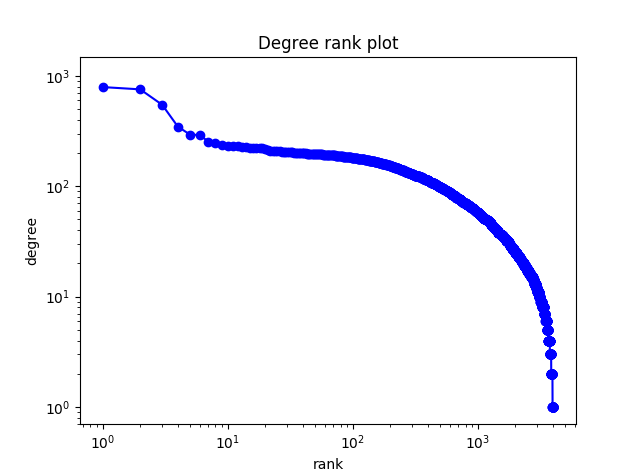
\includegraphics[width=\textwidth,height=\textheight,keepaspectratio]{facebook_degree_distribution}
  \caption{Facebook Degree Distribution}
\end{figure}
\end{column}
\end{columns}
\end{frame}


\begin{frame}
\frametitle{Issues and Improvements}
\begin{itemize}
\item \cite{ghahramani2010} says that there is a narrow band of parameters where kronecker graphs have the interesting properties of real world graphs
\item The largest graph simulated was only of size $2^{12}$ which may not be enough to see the clustering behaviour
\item Might need a larger number of samples from the permutation space to get a better estimate of the likelihood
\item Consider a bayesian approach instead of using maximum likelihood, however this might be prohibitively expensive
\end{itemize}
\end{frame}

%------------------------------------------------


\begin{frame}
\frametitle{Conclusions}
\begin{itemize}
\item Spectral methods can be used to detect planted cliques of size $O(\sqrt{n})$ on a $G(n,p)$
\item Real world networks are more clustered than random graphs
\item Kronecker Matrices can be used to model real world graph structures
\item Training Kronecker Matrices can be quite expensive and may not work on small training sets.
\end{itemize}
\end{frame}

%------------------------------------------------

\begin{frame}
\frametitle{References}
\footnotesize{
\begin{thebibliography}{99}

\bibitem{berthet2013} 
Berthet Quentin,	
Rigollet Philippe,	
{Computational Lower Bounds for Sparse PCA},(2013).

\bibitem{cook2015} 
Cook Alexis B,	
Miller Benjamin A,
{Planted clique detection below the noise floor using low-rank sparse PCA},(2015).

\bibitem{ghahramani2010}
Jon Kleinberg,
Jure Leskovec,
Deepayan Chakrabarti,
Christos Faloutsos,
Zoubin Ghahramani
{Kronecker Graphs: An Approach to Modelling Networks},(2010).

\bibitem{SNAP-dataset}
Jure Leskovec,
Andrej Krevl
{{SNAP Datasets}: {Stanford} Large Network Dataset Collection}


\end{thebibliography}

}
\end{frame}

%------------------------------------------------

\begin{frame}
\Huge{\centerline{The End}}
\end{frame}

%----------------------------------------------------------------------------------------

\end{document} 